\documentclass[aspectratio=169]{beamer}
\usepackage{lmodern}
%\usetheme{Madrid}
%\usecolortheme{giantoak}
\newcommand*\oldmacro{}
\let\oldmacro\insertshorttitle
\renewcommand*\insertshorttitle{\oldmacro\hfill\insertframenumber\,/\,\inserttotalframenumber}
\usepackage[framemethod=tikz]{mdframed}

%\usepackage{beamerthemesplit}
\usepackage{textpos}
\usepackage{pgf}
%\logo{\pgfputat{\pgfxy(0,-.4)}{\pgfbox[right,base]{\includegraphics[height=1.0cm]{logo.jpg}}}}
%\newcommand{\nologo}{\setbeamertemplate{logo}{}}
\usepackage{booktabs}
\usepackage{graphicx}
\theoremstyle{principle}
\newtheorem*{principle}{Design Principle}


\titlegraphic{\includegraphics[width=1.0\paperwidth]{cool-wind-800px.jpg}}

\title{Amendments}
%\author[Jeremy Kedziora]{Wind Data Science Team\\
%\small{Uptake}}
\date{}

\begin{document}

%{
%%\nologo
%\begin{frame}
%    \maketitle
%\end{frame}
%}
%pages 1-7, 8-9, 14-15.


{
%  \usebackgroundtemplate{
\includegraphics[width=1.0\paperwidth]{statistics-review.jpg}}
  \usebackgroundtemplate{
\includegraphics[scale=0.6]{testtubes_stars.png}}
  \begin{frame}[plain]
  
\begin{mdframed}[tikzsetting={draw=white,fill=white,fill opacity=0.6,draw opacity=0.4,
               line width=0pt},backgroundcolor=none,leftmargin=20,
               rightmargin=20,innertopmargin=4pt]
\begin{center}
\Huge \textbf{Experiments vs Observations}
\end{center}
\end{mdframed}

  \end{frame}
}

%most reliant on human cognition
%limited only by cognition
%hypothesis generating scheme often functioning as a gateway into more statistical analysis

%%@@@@@@@@@@@@@@@@@@@@@@@@@@@@@@@@@@@@@@@@@@@@@@@@@
%\begin{frame}
%\frametitle{Napoleon's Progress}
%\begin{center}
%
\includegraphics[scale=0.4]{experiment.png}
%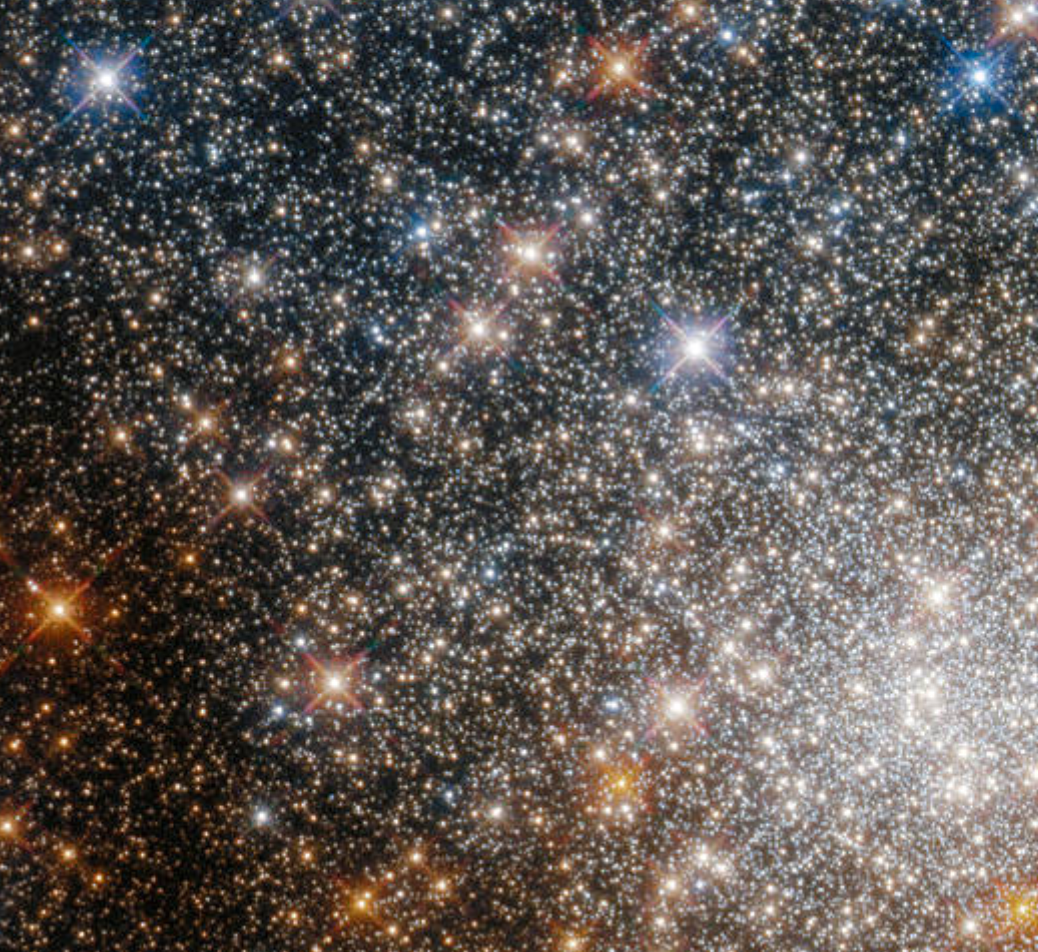
\includegraphics[scale=0.35]{stars.png}
%\end{center}
%
%\end{frame}

%@@@@@@@@@@@@@@@@@@@@@@@@@@@@@@@@@@@@@@@@@@@@@@@@@
\begin{frame}
\frametitle{Today:}

\begin{itemize}
\item Identify the key difference between experimental and observational data;
\bigskip
\bigskip

\item Discuss considerations for experimental data;
\bigskip
\bigskip

\item Introduce observational data.
\end{itemize}

\end{frame}

%@@@@@@@@@@@@@@@@@@@@@@@@@@@@@@@@@@@@@@@@@@@@@@@@@
\begin{frame}
\frametitle{Example 1: the effect of a sentence `toughness' on recividism}

\begin{itemize}
\item \textbf{Question}: does tougher punishment diminish the likelihood that a convict will commit future crimes?
\bigskip
\bigskip

\item \textbf{Data}: a sample of defendants from public records of the DC Superior Court restricted to felony drug offenses/no other offenses;
\begin{itemize}
\item Demographics (name, DOB, race, gender, address);
\item Charge;
\item Judge at time of sentencing;
\item Sentence;
\item Subsequent recividism;
\end{itemize}
\bigskip
\bigskip

\item[]\color{white} \textbf{Random judge assignment}.
\end{itemize}

\end{frame}

%@@@@@@@@@@@@@@@@@@@@@@@@@@@@@@@@@@@@@@@@@@@@@@@@@
\begin{frame}
\frametitle{Example 1: the effect of a sentence `toughness' on recividism}

\begin{itemize}
\item \textbf{Question}: does tougher punishment diminish the likelihood that a convict will commit future crimes?
\bigskip
\bigskip

\item \textbf{Data}: a sample of defendants from public records of the DC Superior Court restricted to felony drug offenses/no other offenses;
\begin{itemize}
\item Demographics (name, DOB, race, gender, address);
\item Charge;
\item Judge at time of sentencing;
\item Sentence;
\item Subsequent recividism;
\end{itemize}
\bigskip
\bigskip

\item \textbf{Random judge assignment}.
\end{itemize}

\end{frame}

%@@@@@@@@@@@@@@@@@@@@@@@@@@@@@@@@@@@@@@@@@@@@@@@@@
\begin{frame}
\begin{center}
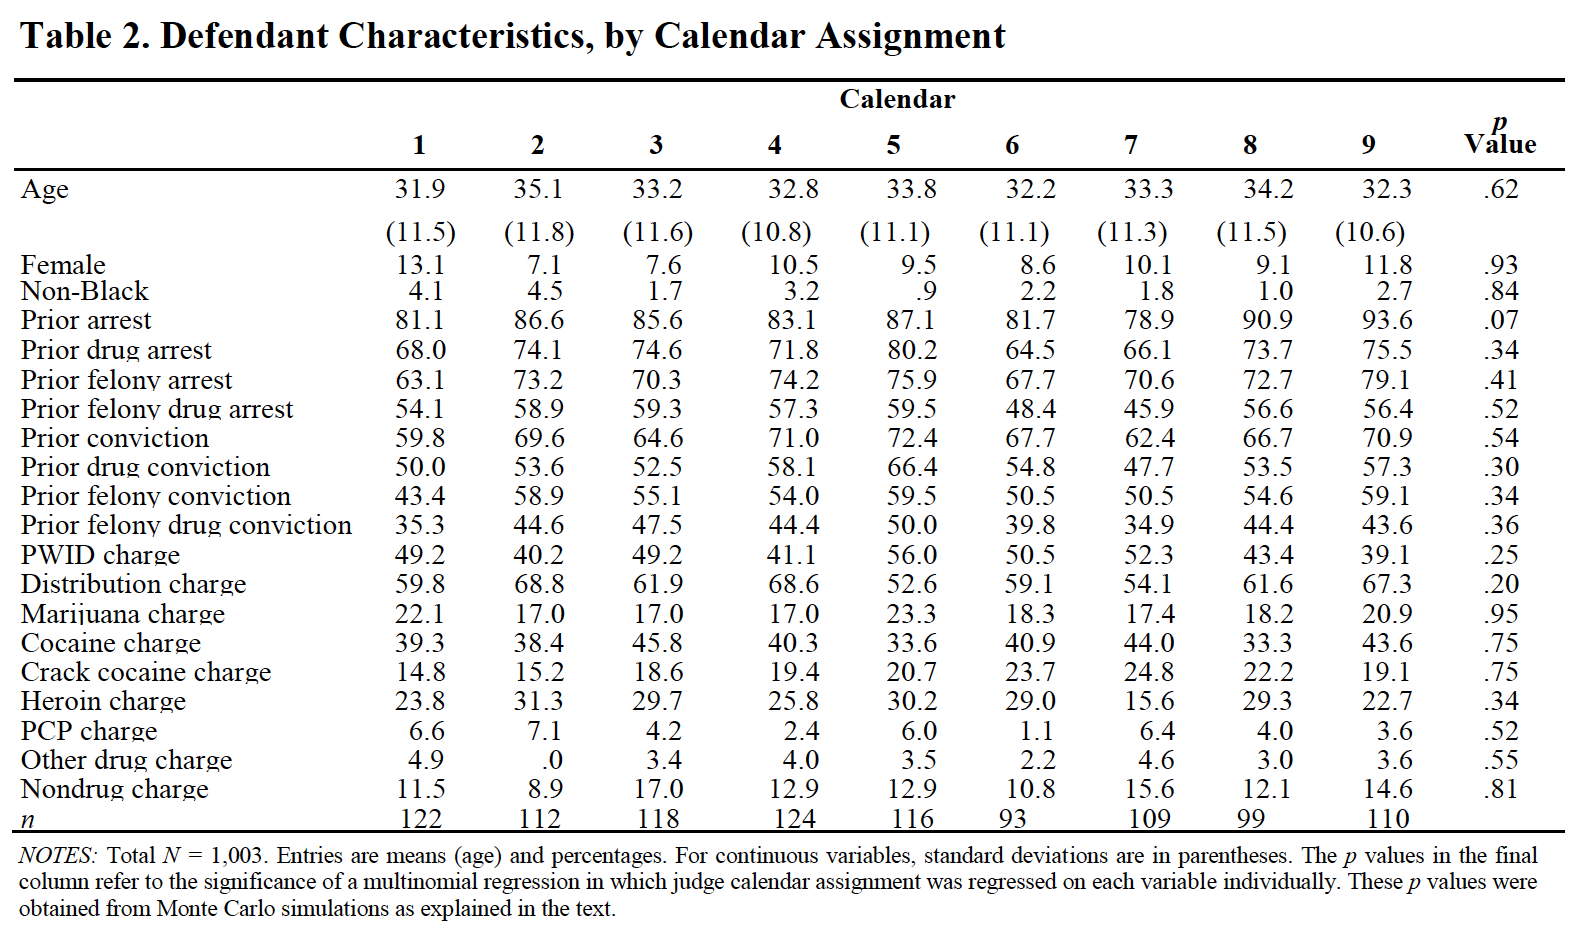
\includegraphics[scale=0.4]{random_judge_assignment.png}
\end{center}

\end{frame}

%@@@@@@@@@@@@@@@@@@@@@@@@@@@@@@@@@@@@@@@@@@@@@@@@@
\begin{frame}
\frametitle{Example 2: explaining civil wars}

\begin{itemize}
\item \textbf{Question}: does the end of the cold war, ethnic nationalism, or something else cause civil wars?
\bigskip
\bigskip
\item \textbf{Data}: a list of civil wars in which:
\begin{itemize}
\item Organized groups fought agents of the state;
\item At least 1k deaths;
\item At least 100 dead on govt side;
\end{itemize}
\bigskip
\item \textbf{Numerous other variables measuring}:
\begin{itemize}
\item political economy (war, GDP, democracy);
\item territorial characteristics (contiguity, mountainous terrain);
\item demographics (population, ethnic/religious fractionalization, pluralism, and polarization)
\end{itemize}
\end{itemize}

\end{frame}

%@@@@@@@@@@@@@@@@@@@@@@@@@@@@@@@@@@@@@@@@@@@@@@@@@
\begin{frame}
\frametitle{Example 2: explaining civil wars}

\begin{itemize}
\item \textbf{Question}: does the end of the cold war, ethnic nationalism, or something else cause civil wars?
\bigskip
\bigskip
\item \textbf{Data}: a list of civil wars in which:
\begin{itemize}
\item Organized groups fought agents of the state;
\item At least 1k deaths;
\item At least 100 dead on govt side;
\end{itemize}
\bigskip
\item \textbf{Numerous other variables measuring}:
\begin{itemize}
\item political economy (war, GDP, democracy);
\item territorial characteristics (contiguity, \textbf{mountainous terrain});
\item demographics (population, ethnic/religious fractionalization, pluralism, and polarization)
\end{itemize}
\end{itemize}

\end{frame}

%@@@@@@@@@@@@@@@@@@@@@@@@@@@@@@@@@@@@@@@@@@@@@@@@@
\begin{frame}
\begin{center}
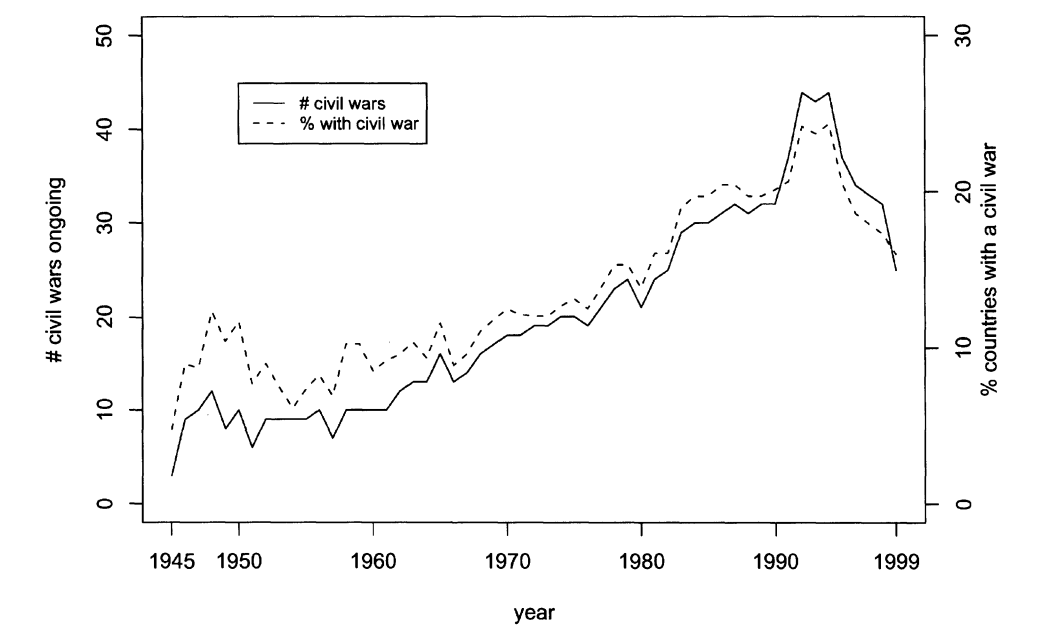
\includegraphics[scale=0.65]{f_and_l.png}
\end{center}

\end{frame}

%@@@@@@@@@@@@@@@@@@@@@@@@@@@@@@@@@@@@@@@@@@@@@@@@@
\begin{frame}
\frametitle{Data Generating Process}

\begin{itemize}
\item A useful (and ubiquitous) construct: \textbf{the data generating process} (DGP) -- the set of all operations that lead to:
\begin{enumerate}
\item the particular observations that appear in the dataset...
\item ...and their structure;
\end{enumerate}
\bigskip
\item Occurs both IRL and at the researcher's desk -- usually we know at most only part of the DGP;
\bigskip
\item[]\color{white} Selected examples:
\begin{enumerate}
\item[]\color{white} Creation of events that could become data -- e.g. only certain countries fight wars;
\item[]\color{white} Selection of selection of population units into the data sample -- e.g. def of civil war;
\item[]\color{white} Categorization/Binarization -- e.g. a Likert scale representation of preference;
\item[]\color{white} Analyst decisions to aggregate, group, or drop data;
\item[]\color{white} Assignment of independent variables to observations (e.g. selection of treatment and control groups);
\end{enumerate}
\bigskip
\item[] \color{white}\textbf{If the researcher controls (5) the data is experimental.}
\end{itemize}

\end{frame}

%@@@@@@@@@@@@@@@@@@@@@@@@@@@@@@@@@@@@@@@@@@@@@@@@@
\begin{frame}
\frametitle{Data Generating Process}

\begin{itemize}
\item A useful (and ubiquitous) construct: \textbf{the data generating process} (DGP) -- the set of all operations that lead to:
\begin{enumerate}
\item the particular observations that appear in the dataset...
\item ...and their structure;
\end{enumerate}
\bigskip
\item Occurs both IRL and at the researcher's desk -- usually we know at most only part of the DGP;
\bigskip
\item Selected examples:
\begin{enumerate}
\item Creation of events that could become data -- e.g. only certain countries fight wars;
\item Selection of selection of population units into the data sample -- e.g. def of civil war;
\item Categorization/Binarization -- e.g. a Likert scale representation of preference;
\item Analyst decisions to aggregate, group, or drop data;
\item \textbf{Assignment of independent variables to observations (e.g. selection of treatment and control groups)};
\end{enumerate}
\bigskip
\item[]\color{white} \textbf{If the researcher controls (5) the data is experimental.}
\end{itemize}

\end{frame}

%@@@@@@@@@@@@@@@@@@@@@@@@@@@@@@@@@@@@@@@@@@@@@@@@@
\begin{frame}
\frametitle{Data Generating Process}

\begin{itemize}
\item A useful (and ubiquitous) construct: \textbf{the data generating process} (DGP) -- the set of all operations that lead to:
\begin{enumerate}
\item the particular observations that appear in the dataset...
\item ...and their structure;
\end{enumerate}
\bigskip
\item Occurs both IRL and at the researcher's desk -- usually we know at most only part of the DGP;
\bigskip
\item Selected examples:
\begin{enumerate}
\item Creation of events that could become data -- e.g. only certain countries fight wars;
\item Selection of selection of population units into the data sample -- e.g. def of civil war;
\item Categorization/Binarization -- e.g. a Likert scale representation of preference;
\item Analyst decisions to aggregate, group, or drop data;
\item \textbf{Assignment of independent variables to observations (e.g. selection of treatment and control groups)};
\end{enumerate}
\bigskip
\item \textbf{If the researcher controls (5) the data is experimental.}
\end{itemize}

\end{frame}

%@@@@@@@@@@@@@@@@@@@@@@@@@@@@@@@@@@@@@@@@@@@@@@@@@
\begin{frame}
\frametitle{``Quiz"}

\begin{itemize}
\item Is example 1 on tough sentencing experimental or observational?
\bigskip
\bigskip

\item Is example 2 on causes of civil wars experimental or observational?
\bigskip
\bigskip

\item Is the example from last time on political fundraising experimental or observational?
\bigskip
\bigskip

\item Is the example on the gender wage gap experimental or observational?
\end{itemize}

\end{frame}

%@@@@@@@@@@@@@@@@@@@@@@@@@@@@@@@@@@@@@@@@@@@@@@@@@
\begin{frame}
\frametitle{Considerations with experiments}

\begin{itemize}
\item A procedure used to \textbf{create} data capable of adjudicating between hypotheses, models, and theories;
\bigskip

\item Independent variables vs dependent variables -- generally known ahead of time;
\bigskip

\item \textbf{Between unit design}: two$+$ groups exposed to one treatment each simultaneously;
\begin{itemize}
\item Requires large numbers of units or sophisticated statistical procedures; 
\end{itemize}
\bigskip
\item \textbf{Within unit design}: units receive a sequence of treatments over time (crossover or longitudinal study);
\begin{itemize}
\item Treatment sequences are randomly assigned -- units `cross over' between treatments; 
\item Each unit serves as their own control;
\item May need to model attrition effects;
\item Order and carryover effects.
\end{itemize}
\end{itemize}

\end{frame}

%@@@@@@@@@@@@@@@@@@@@@@@@@@@@@@@@@@@@@@@@@@@@@@@@@
\begin{frame}
\frametitle{Considerations with experiments: a perfect visit advocate}
\huge
\begin{table}
\begin{tabular}{ c | c | c | c}
Unit & $Y_i(\mbox{visit})$ & $Y_i(\mbox{none})$ & \color{white}$Y_i(\mbox{visit}) - Y_i(\mbox{none})$ \\
\hline
\hline
  1 & \color{gray}\$675 & \textbf{\$150} & \\
  2 & \textbf{\$3600} & \color{gray}\$2500 & \\
  3 & \textbf{\$1900} & \color{gray}\$3300 &Average CE is: \\
  4 & \color{gray}\$2300 & \textbf{\$1000} & \$2129\\
  5 & \textbf{\$2600} & \color{gray}\$2000 & \\
  6 & \color{gray}\$3000 & \textbf{\$0} & \\
  7 & \textbf{\$1950} & \color{gray}\$2500 & \\
\hline
\hline
\end{tabular}
\end{table}

\end{frame}

%@@@@@@@@@@@@@@@@@@@@@@@@@@@@@@@@@@@@@@@@@@@@@@@@@
\begin{frame}
\frametitle{Considerations with experiments: assignment effects}
\begin{itemize}
\item What is the major issue in the `perfect visit advocate' example?
\begin{itemize}
\item[]\color{white} Low contributors are assigned to the control group...
\item[]\color{white} ...so that contributions are related to assignments;
 \end{itemize}
\bigskip
\item How could this happen?  \color{white}Not hard to imagine -- correlate assignment with income:
\begin{itemize}
\item[]\color{white} Control group (no visit) entirely composed of lowest 20\% of income distribution;
\item[]\color{white} Treatment group (visit) entirely composed of highest 20\% of income distribution;
\end{itemize}
\bigskip
\item[]\color{white} How to deal with this?  First steps: large sample, randomized assignment;
\begin{itemize}
\item[]\color{white} As sample size increases the probability of an imbalance in some unobserved characteristic between treatment and control gets arbitrarily low;
\item[]\color{white} Treatment assignment is independent of the potential outcomes.
\end{itemize}
\end{itemize}
\end{frame}

%@@@@@@@@@@@@@@@@@@@@@@@@@@@@@@@@@@@@@@@@@@@@@@@@@
\begin{frame}
\frametitle{Considerations with experiments: assignment effects}
\begin{itemize}
\item What is the major issue in the `perfect visit advocate' example?
\begin{itemize}
\item Low contributors are assigned to the control group...
\item ...so that contributions are related to assignments;
 \end{itemize}
\bigskip
\item How could this happen?  \color{white}Not hard to imagine -- correlate assignment with income:
\begin{itemize}
\item[]\color{white} Control group (no visit) entirely composed of lowest 20\% of income distribution;
\item[]\color{white} Treatment group (visit) entirely composed of highest 20\% of income distribution;
\end{itemize}
\bigskip
\item[]\color{white} How to deal with this?  First steps: large sample, randomized assignment;
\begin{itemize}
\item[]\color{white} As sample size increases the probability of an imbalance in some unobserved characteristic between treatment and control gets arbitrarily low;
\item[]\color{white} Treatment assignment is independent of the potential outcomes.
\end{itemize}
\end{itemize}
\end{frame}

%@@@@@@@@@@@@@@@@@@@@@@@@@@@@@@@@@@@@@@@@@@@@@@@@@
\begin{frame}
\frametitle{Considerations with experiments: assignment effects}
\begin{itemize}
\item What is the major issue in the `perfect visit advocate' example?
\begin{itemize}
\item Low contributors are assigned to the control group...
\item ...so that contributions are related to assignments;
 \end{itemize}
\bigskip
\item How could this happen?  Not hard to imagine -- correlate assignment with income:
\begin{itemize}
\item Control group (no visit) entirely composed of lowest 20\% of income distribution;
\item Treatment group (visit) entirely composed of highest 20\% of income distribution;
\end{itemize}
\bigskip
\item[]\color{white} How to deal with this?  First steps: large sample, randomized assignment;
\begin{itemize}
\item[]\color{white} As sample size increases the probability of an imbalance in some unobserved characteristic between treatment and control gets arbitrarily low;
\item[]\color{white} Treatment assignment is independent of the potential outcomes.
\end{itemize}
\end{itemize}
\end{frame}

%@@@@@@@@@@@@@@@@@@@@@@@@@@@@@@@@@@@@@@@@@@@@@@@@@
\begin{frame}
\frametitle{Considerations with experiments: assignment effects}
\begin{itemize}
\item What is the major issue in the `perfect visit advocate' example?
\begin{itemize}
\item Low contributors are assigned to the control group...
\item ...so that contributions are related to assignments;
 \end{itemize}
\bigskip
\item How could this happen?  Not hard to imagine -- correlate assignment with income:
\begin{itemize}
\item Control group (no visit) entirely composed of lowest 20\% of income distribution;
\item Treatment group (visit) entirely composed of highest 20\% of income distribution;
\end{itemize}
\bigskip
\item How to deal with this?  First steps: \textbf{large sample}, \textbf{randomized assignment};
\begin{itemize}
\item As sample size increases the probability of an imbalance in some unobserved characteristic between treatment and control gets arbitrarily low;
\item Treatment assignment is independent of the potential outcomes.
\end{itemize}
\end{itemize}
\end{frame}

%@@@@@@@@@@@@@@@@@@@@@@@@@@@@@@@@@@@@@@@@@@@@@@@@@
\begin{frame}
\frametitle{Stable Unit Treatment Value Assumption}
\begin{itemize}
\item We estimated the causal effect in a really simple way in the Rubin Causal Model:% -- the difference in average observed outcome between treatment and control groups:
\begin{align*}
\frac{1}{n_T}\sum_iY_i(\mbox{T}) - \frac{1}{n_C}\sum_iY_i(\mbox{C})
\end{align*}
\item \textbf{Fair warning}: should acknowledge that potential outcomes could depend on other stuff, e.g.:
\begin{align*}
Y_1(\hspace{-13.5mm}\underbrace{\mbox{C}}_{\mbox{assignment for unit 1}}\hspace{-13.5mm},\hspace{-5mm}\overbrace{\mbox{T},\mbox{T},\mbox{C},\mbox{T},\mbox{C},\mbox{T}}^{\mbox{assignments for rest}}\hspace{-3mm})
\end{align*}
\item[]\color{white} It is a \textbf{modeling assumption} that we can write:
\begin{align*}
Y_1(\mbox{C},\mbox{T},\mbox{T},\mbox{C},\mbox{T},\mbox{C},\mbox{T}) = Y_1(C);
\end{align*}
This is called the \textbf{Stable Unit Treatment Value Assumption} (SUTVA)!
\end{itemize}
\end{frame}

%@@@@@@@@@@@@@@@@@@@@@@@@@@@@@@@@@@@@@@@@@@@@@@@@@
\begin{frame}
\frametitle{Stable Unit Treatment Value Assumption}
\begin{itemize}
\item We estimated the causal effect in a really simple way in the Rubin Causal Model:% -- the difference in average observed outcome between treatment and control groups:
\begin{align*}
\frac{1}{n_T}\sum_iY_i(\mbox{T}) - \frac{1}{n_C}\sum_iY_i(\mbox{C})
\end{align*}
\item \textbf{Fair warning}: should acknowledge that potential outcomes could depend on other stuff, e.g.:
\begin{align*}
Y_1(\hspace{-13.5mm}\underbrace{\mbox{C}}_{\mbox{assignment for unit 1}}\hspace{-13.5mm},\hspace{-5mm}\overbrace{\mbox{T},\mbox{T},\mbox{C},\mbox{T},\mbox{C},\mbox{T}}^{\mbox{assignments for rest}}\hspace{-3mm})
\end{align*}
\item It is a \textbf{modeling assumption} that we can write:
\begin{align*}
Y_1(\mbox{C},\mbox{T},\mbox{T},\mbox{C},\mbox{T},\mbox{C},\mbox{T}) = Y_1(C);
\end{align*}
This is called the \textbf{Stable Unit Treatment Value Assumption} (SUTVA)!
\end{itemize}
\end{frame}

%@@@@@@@@@@@@@@@@@@@@@@@@@@@@@@@@@@@@@@@@@@@@@@@@@
\begin{frame}
\frametitle{Stable Unit Treatment Value Assumption}
\begin{itemize}
\item What does SUTVA mean?  \color{white}It means:
\begin{itemize}
\item[]\color{white} Potential outcomes for each unit (party member) are not related to treatment assignment for any other unit;
\end{itemize}
\bigskip
\item\color{black} How could this fail to hold? \color{white} Imagine that party members 1 and 2 live in the same household!  Then:
\begin{itemize} 
\item[]\color{white} SUTVA is pretty dubious and...
\item[]\color{white} ...there are four, totally reasonable potential outcomes to think about:
\end{itemize}
\end{itemize}
\Large\vspace{8mm}
\begin{table}
\begin{tabular}{ccccc}
 &&&&\\
&&&&\\
&&&&\\
\end{tabular}
\end{table}

\end{frame}

%@@@@@@@@@@@@@@@@@@@@@@@@@@@@@@@@@@@@@@@@@@@@@@@@@
\begin{frame}
\frametitle{Stable Unit Treatment Value Assumption}
\begin{itemize}
\item What does SUTVA mean?  It means:
\begin{itemize}
\item Potential outcomes for each unit (party member) are not related to treatment assignment for any other unit;
\end{itemize}
\bigskip
\item\color{black} How could this fail to hold? \color{white} Imagine that party members 1 and 2 live in the same household!  Then:
\begin{itemize} 
\item[]\color{white} SUTVA is pretty dubious and...
\item[]\color{white} ...there are four, totally reasonable potential outcomes to think about:
\end{itemize}
\end{itemize}
\Large\vspace{8mm}
\begin{table}
\begin{tabular}{ccccc}
 &&&&\\
&&&&\\
&&&&\\
\end{tabular}
\end{table}

\end{frame}

%@@@@@@@@@@@@@@@@@@@@@@@@@@@@@@@@@@@@@@@@@@@@@@@@@
\begin{frame}
\frametitle{Stable Unit Treatment Value Assumption}
\begin{itemize}
\item What does SUTVA mean?  It means:
\begin{itemize}
\item Potential outcomes for each unit (party member) are not related to treatment assignment for any other unit;
\end{itemize}
\bigskip
\item How could this fail to hold?  Imagine that party members 1 and 2 live in the same household!  Then:
\begin{itemize} 
\item SUTVA is pretty dubious and...
\item ...there are four, totally reasonable potential outcomes to think about:
\end{itemize}
\end{itemize}
\Large
\begin{table}
\begin{tabular}{ c | c | c | c | c}
Unit & $Y_i(\mbox{visit,visit})$ & $Y_i(\mbox{visit},\mbox{none})$ & $Y_i(\mbox{none},\mbox{visit})$ & $Y_i(\mbox{none},\mbox{none})$ \\
\hline
\hline
  1 & \$675 & ? & ? & ? \\
  2 & \vdots & \vdots & \vdots & \vdots \\
\hline
\hline
\end{tabular}
\end{table}

\end{frame}

%@@@@@@@@@@@@@@@@@@@@@@@@@@@@@@@@@@@@@@@@@@@@@@@@@
\begin{frame}
\frametitle{Stable Unit Treatment Value Assumption}
\begin{itemize}
\item How many causal effects are there?
\begin{align*}
Y_i(\mbox{visit},\mbox{none}) &- Y_i(\mbox{none},\mbox{none}) \hspace{5mm}\mbox{ CE of treatment on 1 given 2 untreated}\\
Y_i(\mbox{none},\mbox{visit}) &- Y_i(\mbox{none},\mbox{none}) \hspace{5mm}\mbox{ Spillover for a not treated 1 given 2 treated}\\
Y_i(\mbox{visit,visit}) &- Y_i(\mbox{none},\mbox{visit}) \hspace{6mm}\mbox{ CE of treatment on 1 given 2 treated}\\
Y_i(\mbox{visit,visit}) &- Y_i(\mbox{visit},\mbox{none}) \hspace{6mm}\mbox{ Spillover for a treated 1 given 2 treated}
\end{align*}

\item[] \color{white}\href{https://community.lawschool.cornell.edu/wp-content/uploads/2020/12/Green-presentation-on-SUTVA-for-CELS.pdf}{\underline{Spillover examples}} when SUTVA does not hold:
\begin{itemize}
\item[] \color{white} \textbf{Contagion} -- the effect of vaccination on probability of sickness depends on vaccination of others;
\item[] \color{white} \textbf{Displacement} -- intervention intended to suppress something in one location moves it to other locations;
\item[] \color{white} \textbf{Communication} -- informational interventions may spread across people;
\item[] \color{white} \textbf{Comparison} -- an intervention that assists the treatment group may change how the control groups views their conditions;
\item[] \color{white} \textbf{Persistence/memory} -- in a within subject study, outcomes for a unit are tracked over time, meaning that treatments could persist across time periods;
\end{itemize}
\end{itemize}
\end{frame}

%@@@@@@@@@@@@@@@@@@@@@@@@@@@@@@@@@@@@@@@@@@@@@@@@@
\begin{frame}
\frametitle{Stable Unit Treatment Value Assumption}
\begin{itemize}
\item How many causal effects are there?
\begin{align*}
Y_i(\mbox{visit},\mbox{none}) &- Y_i(\mbox{none},\mbox{none}) \hspace{5mm}\mbox{ CE of treatment on 1 given 2 untreated}\\
Y_i(\mbox{none},\mbox{visit}) &- Y_i(\mbox{none},\mbox{none}) \hspace{5mm}\mbox{ Spillover for a not treated 1 given 2 treated}\\
Y_i(\mbox{visit,visit}) &- Y_i(\mbox{none},\mbox{visit}) \hspace{6mm}\mbox{ CE of treatment on 1 given 2 treated}\\
Y_i(\mbox{visit,visit}) &- Y_i(\mbox{visit},\mbox{none}) \hspace{6mm}\mbox{ Spillover for a treated 1 given 2 treated}
\end{align*}

\item \href{https://community.lawschool.cornell.edu/wp-content/uploads/2020/12/Green-presentation-on-SUTVA-for-CELS.pdf}{\color{blue}\underline{Spillover examples}} \color{black} when SUTVA does not hold:
\begin{itemize}
\item \textbf{Contagion} -- the effect of vaccination on probability of sickness depends on vaccination of others;
\item \textbf{Displacement} -- intervention intended to suppress something in one location moves it to other locations;
\item \textbf{Communication} -- informational interventions may spread across people;
\item \textbf{Comparison} -- an intervention that assists the treatment group may change how the control groups views their conditions;
\item \textbf{Persistence/memory} -- in a within subject study, outcomes for a unit are tracked over time, meaning that treatments could persist across time periods;
\end{itemize}
\end{itemize}
\end{frame}




%%@@@@@@@@@@@@@@@@@@@@@@@@@@@@@@@@@@@@@@@@@@@@@@@@@
%\begin{frame}
%\frametitle{An example: the effect of sentence `toughness' on recividism}
%
%\begin{itemize}
%\item Assumptions:
%\begin{itemize}
%\item Judges have different sentencing propensities;
%\item Judge influences recividism only through sentence;
%\item Sentence of one defendent does not impact any other defendent (SUTVA);
%\end{itemize}
%\bigskip
%\item Blar.
%\end{itemize}
%
%\end{frame}

%@@@@@@@@@@@@@@@@@@@@@@@@@@@@@@@@@@@@@@@@@@@@@@@@@
\begin{frame}
\frametitle{Characteristics of observation}

\begin{itemize}
\item A procedure used to \textbf{collect} data capable of adjudicating between hypotheses, models, and theories;
\bigskip
\bigskip

\item Can be used for exploratory purposes.
\bigskip
\bigskip

\item Why not just use experiments?  \color{white}In some fields, the independent variables under study are not subject to manipulation, and so not subject to experiments, e.g.:
\begin{itemize}
\item[]\color{white} Astronomy (lack of influence);
\item[]\color{white} Epidemiology (ethics);
\item[]\color{white} International relations (both!);
\end{itemize}

\end{itemize}

\end{frame}

%@@@@@@@@@@@@@@@@@@@@@@@@@@@@@@@@@@@@@@@@@@@@@@@@@
\begin{frame}
\frametitle{Characteristics of observation}

\begin{itemize}
\item A procedure used to \textbf{collect} data capable of adjudicating between hypotheses, models, and theories;
\bigskip
\bigskip

\item Can be used for exploratory purposes.
\bigskip
\bigskip

\item Why not just use experiments?  In some fields, the independent variables under study are not subject to manipulation, and so not subject to experiments, e.g.:
\begin{itemize}
\item Astronomy (lack of influence);
\item Epidemiology (ethics);
\item International relations (both!);
\end{itemize}

\end{itemize}

\end{frame}

%%@@@@@@@@@@@@@@@@@@@@@@@@@@@@@@@@@@@@@@@@@@@@@@@@@
%\begin{frame}
%\frametitle{Validity}
%
%\begin{itemize}
%\item Blar;
%\bigskip
%\item Blar;
%\bigskip
%\item Blar;
%\bigskip
%\item Blar;
%\bigskip
%\item Blar;
%\bigskip
%\item Blar.
%\end{itemize}
%
%\end{frame}

%@@@@@@@@@@@@@@@@@@@@@@@@@@@@@@@@@@@@@@@@@@@@@@@@@
\begin{frame}

\begin{center}
\Huge\textbf{Why should we care?}\\
\bigskip
\bigskip
\large We will work with both types of data this semester and the methods applied to analyze each will be somewhat different.\\
\end{center}

\end{frame}



\end{document}






